\chapter{1. A construção da integração mundial}

\coment{Este módulo foi estruturado seguindo uma linha temporal que explicita o
desenvolvimento do processo de globalização e, ao mesmo tempo, mobiliza
os conteúdos necessários para a efetivação do eixo e das habilidades
associadas.\\
Habilidades da BNCC: EF09GE05, EF09GE06, EF09GE09.}

\colorsec{Eixo de conhecimento do SAEB}

\begin{itemize}
\item Tempo e espaço: fontes e formas de representação
\end{itemize}

\conteudo{O desenvolvimento da configuração de mundo atual é resultado de longo processo histórico, que não pode ser compreendido sem considerarmos o papel da colonização e do desenvolvimento do capitalismo, sistema econômico que hoje integra todo o mundo em sua lógica.

Tal processo possui íntima relação com o desenvolvimento da cartografia, que, desde suas bases na Antiguidade, desenvolveu-se seguindo os rumos das grandes navegações, o que torna evidente também quanto a Antiguidade Clássica relaciona-se com a Europa que colonizou o mundo.

A globalização integrou o mundo por meio do desenvolvimento tecnológico e da consolidação do capitalismo a nível global, conseguindo estabelecer padrões gerais de consumo, cultura e organização social. Tal interação assenta-se no predomínio das lógicas ocidentais do mundo gestadas na Europa.}

\coment{Ao longo das atividades, ficará perceptível que as questões estão
encadeadas, de modo que o conteúdo vai se
articulando por meio de atividades interpretativas que mobilizam também o
conteúdo previsto para ser visto ao longo dos quatro Anos Finais do Ensino
Fundamental. Essa é uma forma que facilita a compreensão
do aluno ao seguir uma estrutura que remete a uma sequência de aulas.}


\colorsec{Atividades}

\begin{quote}
Os mapas medievais ``T e O'' originaram-se da descrição do mundo na
obra \emph{Etymologia}, de Isidoro de Sevilha. Este conceito de
cartografia medieval representa apenas o hemisfério norte de uma Terra
esférica, dedução feita a partir da projeção da porção habitada do mundo
conhecida nos tempos romanos e medievais.

\begin{figure}[htpb!]
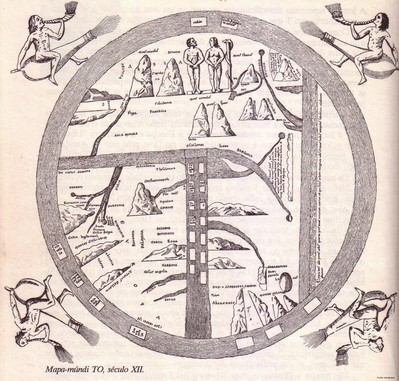
\includegraphics[width=2.88577in,height=2.76032in]{./imgs/img1.jpg}
\caption{Fonte: /www.geografia.seed.pr.gov.br/modules/galeria/detalhe.php?foto=401\&evento}
\end{figure}

O ``T'' é o Mediterrâneo
dividindo em três contimentes: Europa, Ásia e África, sendo o ``O'' um
Oceano circundante. Jerusalém era usualmente representada no centro do
mapa e a Ásia surgia do tamanho da soma dos outros dois continentes.
Porque o Sol nascia a leste, e o Paraíso (jardim do Éden) era geralmente
representado como sendo na Ásia, estando, dessa maneira, situada na
porção superior do mapa.

\fonte{Secretaria da Educação. Mapa T O. Disponível em: \emph{www.geografia.seed.pr.gov.br/modules/galeria/detalhe.php?foto=401\&evento}. Acesso em: 19 fev. 2023.}
\end{quote}

\num{1} Mapas são representações não apenas do espaço geográfico, mas também
de ideias e concepções de mundo. No caso do mapa T O, qual era a
concepção de mundo em sua base?

\linhas{4}

\coment{Como o mapa representava apenas a porção do planeta conhecida pelos
elaboradores, a concepção de mundo deles acreditava que não existia mais
superfície terrestre para além das áreas conhecidas, sendo esse conjunto
o único tipo de mundo aceito como existente.}

\num{2} O mapa T O era um mapa medieval, de uma época em que não estavam prontas as
bases da cartografia como a conhecemos hoje. Circule os nomes dos elementos que estão ausentes nesse mapa, mas que devem
\textbf{obrigatoriamente} existir nos mapas contemporâneos.

\begin{multicols}{2}
\red{LEGENDA}

FIGURAS

\red{TÍTULO}

SIMBÓLICAS

TRAÇADO DE ESTRADAS
\end{multicols}

\coment{Os mapas contemporâneos precisam dispor de alguns elementos básicos,
como título, legenda, escala e orientação. Esses elementos permitem
identificarmos o tema, como ele está sendo representado, comparação
entre o tamanho do mapa e o tamanho da área representada e a disposição
dos elementos espaciais no espaço.}

\num{3} Leia os dois textos a seguir.

\textbf{TEXTO 1}
\begin{quote}

{[}...{]}

Durante muitos séculos, os mapas foram um privilégio da elite.
Apenas reis, nobres, alto clero, grandes navegadores e armadores de
expedições marítimas, tinham acesso a esse tipo de informação. Somente a
partir da invenção da imprensa, na segunda metade do século XV, os mapas
puderam ser mais amplamente utilizados.

{[}...{]}

\fonte{IBGE. \emph{Atlas Geográfico Escolar na
Internet.} Disponível em:
\emph{https://atlasescolar.ibge.gov.br/conceitos-gerais/historia-da-cartografia/a-era-dos-descobrimentos-sec-xv-a-xviii.html}.
Acesso em: 19 fev. 2023.}
\end{quote}

\textbf{TEXTO 2}
\begin{quote}

Depois de inventar os tipos móveis, Gutenberg ajudou a dar início
a uma revolução cultural. Os padrões de impressão definidos por ele
consolidaram-se de tal forma que se mantiverem sem grandes alterações
até o século XVIII. Por isso, o nome de Gutenberg está na lista dos
personagens mais influentes da história. Em 2000, por exemplo, alguns
meios de comunicação o definiram como o \textbf{homem do milênio}.

\fonte{Fonte de pesquisa: National Geographic Portugal. Johannes Gutenberg e os princípios da impressão. Disponível
em: \emph{https://nationalgeographic.pt/historia/grandes-reportagens/3086-johannes-gutenberg-e-os-principios-da-impressao}.
Acesso em: 19 fev. 2023.}
\end{quote}

Agora, leia esta afirmativa:

\textit{A popularização e o aperfeiçoamento dos mapas estão diretamente relacionados
ao avanço técnico ocorrido às vésperas do mercantilismo.}

Explique se você concorda com essa afirmativa ou se você discorda dela.

\linhas{4}

\coment{A articulação entre os textos deixa claro que os mapas deixaram de ser
privilégio da elite apenas após a capacidade de impressão em massa dos
mapas ser atingida, ou seja, temos uma inovação técnica associada ao
desenvolvimento cartográfico.}

\num{4} Leia o texto.

\begin{quote}
\textbf{Mercantilismo}

{[}...{]}

A obtenção de riqueza no mercantilismo poderia se dar de diversas
maneiras. O Estado poderia cobrar impostos da população, vender cargos
públicos e títulos de nobreza, confiscar bens, ceder privilégios
comerciais para um determinado grupo em troca de compensação financeira
(monopólios), exportar mercadorias, saquear em contextos de guerra,
cobrar taxas alfandegárias, realizar ações de pirataria
etc.

{[}...{]}

Um acontecimento extremamente importante para o sucesso
dessas práticas econômicas entre as nações europeias foi o
colonialismo.

O colonialismo foi fundamental para os Estados europeus, pois
permitiu que eles explorassem inúmeros recursos de suas colônias e os
enviassem para a Europa. Isso também possibilitou que essas colônias
fossem transformadas em consumidores compulsórios de suas metrópoles,
por conta do exclusivismo comercial.

{[}...{]}

\fonte{Daniel Neves Silva. História do Mundo. Mercantilismo. Disponível em:
\emph{https://www.historiadomundo.com.br/idade-moderna/mercantilismo.htm}.
Acesso em: 19 fev. 2023.}
\end{quote}

Na Idade Média, considerava-se o mundo como
restrito a Europa, Ásia e África. A partir da leitura do texto, o que
muda na visão europeia sobre a extensão do mundo a partir do
mercantilismo?

\linhas{4}

\coment{Em contraposição à ideia de um mundo restrito a Ásia, Europa e África, a
colonização marcou também a ``descoberta'' do continente americano pelos
europeus, o que ampliou o mundo conhecido até então.}

\num{5} A globalização é caracterizada pela integração de fluxos comerciais,
populacionais, culturais e sociais. Sobre o assunto, analise estas informações:

\begin{itemize}
  \item \textbf{1500-1840}: a velocidade média das carruagens e dos barcos a vela
  era de 16 km/h;
  \item \textbf{1850-1930}: a velocidade média das locomotivas a vapor era de 100 km/h,
  enquanto a dos barcos a vapor era de 57 km/h;
  \item \textbf{Década de 1950}: os jatos de passageiros alcançavam velocidades entre
  480 e 640 km/h;
  \item \textbf{Década de 1960}: os jatos de passageiro alcançavam velocidades entre
  800 e 1.100 km/h.
\end{itemize}

Como essas informações relacionam-se com a globalização?

\linhas{5}

\coment{Com o passar do tempo, os meios de transporte se desenvolveram, o que diminuiu
os tempos de locomação entre dois pontos do mundo, como se as distâncias no planeta tivessem
também diminuído. Com isso, veio a maior rapidez nos deslocamentos de pessoas e mercadorias,
uma característica da globalização.}

\num{7}

\begin{quote}
\textbf{Globalização}

{[}...{]}

A origem dos termos \emph{sociedade global}
e \emph{globalização} é anterior ao triunfo político
da \emph{globalização neoliberal}; data
de finais dos anos 1960 e deve ser creditada a MacLuhan e a Bzezinski
{[}...{]}. {[}...{]} Brzezinski colocou em circulação as expressões \emph{cidade global} e
\emph{sociedade global} para designar a nova reconfiguração globalizada do
nosso hábitat, operada pelas redes tecnotrônicas (termo introduzido por
ele para designar a conjugação do computador, da TV e da rede de
telecomunicação). O protótipo dessa ``sociedade global'' eram os [Estados Unidos],
centro propulsor da revolução ``tecnotrônica'' mundial que oferecia ao
mundo o ``único modelo global de modernidade'', com os correspondentes
``padrões de comportamento e valores universais''.

{[}...{]}

\fonte{Ramon Peña Castro. Dicionário da
educação profissional em saúde. Globalização. Disponível em:
\emph{http://www.sites.epsjv.fiocruz.br/dicionario/verbetes/glo.html}.
Acesso em: 19 fev. 2023.}
\end{quote}

Segundo o texto, como o advento de novas tecnologias de comunicação
ajudou a integrar o conjunto dos países?

\linhas{5}

\coment{Os meios de comunicação tornam possível a transmissão de informações
para lugares distantes, e não apenas informação, mas também ideias,
modelos de vida e manifestações culturais. Quem domina os meios de
comunicação também domina o que é transmitido, ajudando a moldar os
discursos dominantes.}

\num{8} Leia o texto.

\begin{quote}
\textbf{Saiba um pouco mais sobre a história do movimento Manguebeat}

O manguebeat surgiu em Pernambuco, como um movimento de
contracultura. Ele era formado principalmente por jovens que usavam a
música como uma forma de inclusão social {[}...{]}.

O nome surgiu de uma fusão da palavra \emph{mangue} com a palavra \emph{bit}
(unidade de memória de computadores). Assim como o mangue, que é rico em
sua biodiversidade, o manguebeat criou uma cena musical bem
diversificada, misturando ritmos regionais pernambucanos como: maracatu,
frevo, ciranda e caboclinho, pop, rap, hip hop e música eletrônica. O
movimento se beneficiou de ferramentas tecnológicas recém-surgidas, o
que proporcionou a gravação das músicas em ``home studios'', e do
surgimento da internet, principal fonte de divulgação.

Diversos grupos se destacaram: Mundo Livre S/A, Chico Science \&
Nação Zumbi, Sheik Tosado, Mestre Ambrósio, Faces do Subúrbio, Eddie,
Via Sat, Querosene Jacaré e Jorge Cabeleira.

{[}...{]}

\fonte{TV UNESP. Saiba um pouco mais sobre a história do movimento Manguebeat.
Disponível em: \emph{https://tv.unesp.br/old/616}. Acesso
em: 19 fev. 2023.}
\end{quote}

Músicas como pop, rap e eletrônica possuem origens diversas para além das
fronteiras brasileiras. Nesse sentido, o que a mistura desses ritmos por
grupos brasileiros pode dizer sobre a globalização?

\linhas{5}

\coment{A fusão de ritmos demonstra que a música não se restringe mais aos
países e aos territórios em que são criadas, espalhando-se pelos meios
de comunicação, o que permite também a apropriação por outros grupos.
Isso gera uma integração cultural característica da globalização.}

\num{9} Leia as informações a seguir.

\textbf{I. Os 10 produtos mais exportados pelo Brasil em 2022 para a China}

\begin{enumerate}
\item Soja;
\item Minério de ferro e seus concentrados;
\item Óleos brutos de petróleo ou de minerais betuminosos;
\item Açúcares e melaços;
\item Carne bovina;
\item Farelos de soja e outros alimentos para animais;
\item Celulose;
\item Milho não moído;
\item Produtos manufaturados;
\item Carnes de aves e suas miudezas comestíveis, frescas, refrigeradas ou congeladas.
\end{enumerate}

\fonte{Fonte de pesquisa: Fazcomex, 22 nov. 2022. Disponível em:
\emph{https://www.fazcomex.com.br/comexstat/asia/exportacao-china/}.
Acesso em: 03 abr. 2023.}

\textbf{II. Os principais produtos importados pelo Brasil da China}

\begin{enumerate}
\item
  Equipamentos de telecomunicações;
\item
  Válvulas e tubos termiônicas;
\item
  Compostos organo-inorgânicos;
\item
  Produtos manufaturados;
\item
  Adubos ou fertilizantes;
\item
  Medicamentos e produtos farmacêuticos, exceto veterinários;
\item
  Máquinas e aparelhos elétricos;
\item
  Peças e acessórios para escritório;
\item
  Aparelhos elétricos para ligação;
\item
  Máquinas de energia elétrica;
\end{enumerate}

\fonte{Fonte de pesquisa: Fazcomex, 22 mar. 2023. Disponível em:
\emph{https://www.fazcomex.com.br/comex/produtos-importados-da-china-para-o-brasil/}.
Acesso em: 03 abr. 2023.}

\num{a} Quem vende mais produtos industrializados, Brasil ou China?

\linhas{1}

\coment{A China vende mais produtos industrializados do que o Brasil.}

\num{b} O que isso revela sobre a relação entre os dois países?

\linhas{3}

\coment{Isso mostra que o parque industrial chinês è mais desenvolvido e que a
indústria tem menor participação na composição econômica do Brasil.}

\num{10} A produção industrial mundial concentra-se na América do Norte, no leste
da Ásia e no oeste da Europa. Sobre isso, explique o significado desta afirmativa:

\begin{quote}
A globalização é marcada por um pequeno grupo de países produtores e um
imenso grupo de consumidores.
\end{quote}

\linhas{6}

\coment{A produção industrial é monopólio de poucos países, ou seja, eles
produzem aquilo de mais avançado existente até hoje, enquanto o restante
do mundo apenas consome os produtos e reproduzem a tecnologia fabril
oriunda de outros países.}

\colorsec{Treino}

\num{1} Leia o texto.

\begin{quote}
\textbf{O mundo ocidental e o mundo oriental}

De modo geral, podemos definir o mundo oriental como a porção
da Terra formada pelas nações da Ásia e do Oriente Médio, enquanto o
mundo ocidental engloba a Europa e grande parte dos territórios que
foram colonizados pelos europeus, notadamente a América, a Austrália e a
Nova Zelândia.

{[}...{]}

\fonte{Conexão Escola. Prefeitura de Goiânia. Disponível em:
\emph{https://sme.goiania.go.gov.br/conexaoescola/eaja/geografia-mundo-oriental-e-mundo-ocidental/}.
Acesso em: 20 fev 2023.}
\end{quote}

Identifica-se no texto que o mundo ocidental corresponde

\begin{escolha}
\item
  ao conjunto dos países europeus.
\item
  às sociedades que seguem o Islamismo.
\item
  aos territórios localizados no Hemisfério Oeste.
\item
  aos países condicionados pela cultura europeia.
\end{escolha}

\coment{BNCC: EF09GE06 -- Associar o critério de divisão do mundo em Ocidente e
Oriente com o Sistema Colonial implantado pelas potências europeias.

a) Incorreta. A porção colonizada pela Europa também
  integra o mundo ocidental. b) Incorreta: O Islamismo é uma religião presente majoritariamente no
  mundo oriental. c) Incorreta. Essa concepção considera apenas a posição dos países no
  globo, mas a concepção de mundo ocidental considera principalmente o
  aspecto cultural. d) Correta. O mundo ocidental é entendido como o conjunto dos países e
  das sociedades que foram condicionados em alguma medida pela sociedade
  europeia ocidental, e isso inclui a própria Europa e todo o conjunto de
  países colonizados pelos europeus, como o continente americano, a
  Austrália e a Nova Zelândia.}

\num{2} Leia o texto.

\begin{quote}
\textbf{História da cartografia: a Idade Média}

Isodoro (570-636 d.C.), bispo de Sevilha, criou o mapa
etimologias, também conhecido como mapa T-O. Esse mapa esquemático tinha
o seguinte significado: o ``T'' representava os três cursos d'água que
dividiam o ecúmero, o Mediterrâneo, que separa a Europa da África; o
Nilo, separando a África da Ásia; e o Don, entre a Ásia e a Europa. O
ecúmero teria sido dividido por Noé entre seus três filhos após o
dilúvio. Além disso, o ``T'' também simbolizava a cruz e na sua junção
estaria localizada Jerusalém, centro do mundo. Esses mapas, em sua
maioria, eram circulares e emoldurados por um grande oceano.

{[}...{]}

\fonte{IBGE. Atlas escolar. Disponível em:
\emph{https://atlasescolar.ibge.gov.br/conceitos-gerais/historia-da-cartografia/a-idade-media.html}.
Acesso em: 20 fev. 2023.}
\end{quote}

A concepção de um mundo restrito a Europa, Ásia e África representada
nos mapas T-O explica-se

\begin{escolha}
\item
  pelo restrito conhecimento astronômico.
\item
  pela inexistência de satélites que fotografassem do espaço.
\item
  pelo desconhecimento de outros locais por parte dos europeus.
\item
  pela crença de existência em um mundo habitado por seres míticos.
\end{escolha}

\coment{BNCC: EF09GE05 -- Analisar fatos e situações para compreender a
integração mundial (econômica, política e cultural), comparando as
diferentes interpretações: globalização e mundialização.

a) Incorreta. A astronomia é uma ciência que se desenvolve desde o Egito
  e a Grécia antiga. b) Incorreta. Os primeiros mapas não dependiam de satélites para sua
  confecção e baseavam-se em dados de navegação, esquemas matemáticos e
  idealizações do mundo. c) Correta. O mapa T-O representava apenas a porção do mundo conhecida
  por seus elaboradores; assim todo o continente americano ficava de
  fora dessa representação, pois apenas o mundo conhecido era
  representado. d) Incorreta. Apesar da existência de lendas sobre a existência de seres
  míticos para além do mundo conhecido, essas lendas só apareceram mais
  fortemente durante as grandes navegações.}

\num{3} Leia o texto.

\begin{quote}
\textbf{Fórum Social Mundial}

Conforme define sua Carta de Princípios, o Fórum Social Mundial
é um espaço internacional para a reflexão e organização de todos os que
se contrapõem à globalização neoliberal e estão construindo alternativas
para favorecer o desenvolvimento humano e buscar a superação da
dominação dos mercados em cada país e nas relações internacionais.
{[}...{]}

\fonte{Espaço Fórum Social Mundial Porto Alegre. Fórum Social Mundial. Disponível em:
\emph{http://forumsocialportoalegre.org.br/forum-social-mundial/}. Acesso
em: 20 fev. 2023.}
\end{quote}

A justificativa apresentada pelo texto valida a ideia de que a
globalização seria um sistema mundial baseado

\begin{escolha}
\item
  na integração dos sistemas políticos nacionais.
\item
  na solidariedade mútua entre a comunidade global.
\item
  no desenvolvimento pleno dos antigos países colonizados.
\item
  no domínio territorial por parte dos mercados desenvolvidos.
\end{escolha}

\coment{BNCC: EF09GE05 -- Analisar fatos e situações para compreender a
integração mundial (econômica, política e cultural), comparando as
diferentes interpretações: globalização e mundialização.

a) Incorreta. Não existe no texto a contraposição à ideia apresentada
  pela alternativa. b) Incorreta. A menção à busca pelo desenvolvimento
  humano e a crítica ao neoliberalismo evidenciam que o Fórum critica a
  falta dos aspectos apresentados na alternativa. c) Incorreta. O fato de se reivindicar maior desenvolvimento humano é uma
  evidência que atesta o não desenvolvimento dos países
  subdesenvolvidos. d) Correta. No texto, critica-se a política neoliberal, ou seja, aquela
  que coloca nos mercados e nas empresas financeiras o centro das políticas
  econômicas, permitindo que o capital financeiro de países estrangeiros
  possa agir sem regulamentação em todo o mundo.}


\chapter{2. Energia e circuitos produtivos}

\coment{Este módulo parte do entendimento do conceito de energia para embasar
um raciocínio que sintetiza como ocorre o intermédio da relação
sociedade-natureza por meio de seus circuitos que exploram os recursos
naturais. O mesmo conceito serve de alicerce para a compreensão dos
fenômenos naturais e sua relação com as intervenções humanas na
paisagem. Três pontos são fundamentais para o trabalho pedagógico deste módulo, que se resumem ao entendimento das Revoluções Industriais como um processo com o qual se complexificaram as tecnologias de produção de energia e de produção industrial, o que resultou na criação de estruturas urbanas que centralizavam cada vez mais a população e o funcionamento econômico. Essa concepção é necessária para que os alunos consigam compreender e resolver as primeiras atividades.
Habilidade da BNCC: EF09GE18.}


\colorsec{Eixo de conhecimento do SAEB}

\begin{itemize}
\item Natureza e questões socioambientais.
\end{itemize}

\conteudo{Não conseguimos compreender a atual configuração do mundo globalizado e todos os seus problemas e desafios sem considerarmos o papel da industrialização de base ocidental na conformação desse mundo, sendo a urbanização contemporânea filha legítima das Revoluções Industriais.

Esse foi o mesmo processo que gerou um desequilíbrio entre a exploração dos recursos naturais e o tempo de renovação da natureza, demandando um direcionamento da energia para a produção industrial, a qual exige a completa desestruturação das reservas materiais da natureza.

A transferência da energia armazenada na natureza para a atmosfera gerou e gera, por sua vez, profundas alterações no ciclo climático, o que mudou os rumos dados pela natureza à superfície terrestre.

Por fim, a industrialização a nível global provocou a paulatina alienação do conjunto da sociedade de sua base natural, sendo necessária a reavaliação de nossa relação com o espaço terrestre.}

\colorsec{Atividades}

\num{1} Observe os detalhes da imagem a seguir.

\begin{figure}[htpb!]

\includegraphics[width=\textwidth]{./imgs/img5.jpg}
\caption{Fonte: https://pt.wikipedia.org/wiki/Revolu\%C3\%A7\%C3\%A3o\_Industrial\#/media/Ficheiro:Griffiths'\_Guide\_to\_the\_iron\_trade\_of\_Great\_Britain\_an\_elaborate\_review\_of\_the\_iron\_(and)\_coal\_trades\_for\_last\_year,\_addresses\_and\_names\_of\_all\_ironmasters,\_with\_a\_list\_of\_blast\_furnaces,\_iron\_(14761790294).jpg. Paisagem inglesa da década de 1870.}
\end{figure}


\num{a} Como podemos relacionar as chaminés à poluição da natureza?

\linhas{8}

\coment{As chaminés emitem fumaça oriunda da queima de combustíveis e leva para a
atmosfera substâncias que podem intoxicar seres humanos e bichos, além de
emitir gases que modificam o funcionamento da atmosfera, como o dióxido de carbono.}

\num{b} Que tipo de energia é utilizada nessas fábricas: fóssil, solar, hidráulica ou eólica? Explique.

\linhas{8}

\coment{A Primeira Revolução Industrial pautou-se pela queima do
carvão mineral, um combustível fóssil, originado da mineralização de
restos vegetais. Sua queima esquentava a água para gerar vapor capaz de
mover máquinas rudimentares.}

\num{2} Ainda sobre a imagem presente na atividade anterior, percebe-se, na paisagem retratada, a existência de elementos rurais ao lado das fábricas.
Sobre esse fato, analise as afirmativas e marque V para o que for verdadeiro e F para o que for falso.

\begin{boxlist}
\item As cidades industriais intensificaram a transformação da natureza e
do meio rural. \coment{V}

\item O surgimento das indústrias centralizou a economia nas cidades. \coment{V}

\item A presença de fazendas nas cidades exemplifica o convívio duradouro
entre os tipos de produção. \coment{F}

\item A natureza repõe seus recursos mais rápido do que a necessidade
industrial. \coment{F}
\end{boxlist}

\coment{A urbanização praticamente eliminou as atividades rurais dos centros
urbanos, concentrando-as na zona rural. A produção industrial demanda
recursos em uma velocidade superior àquela em que natureza os produz -- o
carvão, por exemplo, leva ao menos 400 milhões de anoa para se formar e pode
ser esgotado em algumas décadas.}

\num{3} Leia o texto a seguir.

\begin{quote}
\textbf{O que é energia}
Apesar de ser usada em vários contextos diferentes, o uso
científico da palavra \emph{energia} tem um significado bem definido e preciso:

Potencial inato para executar trabalho ou realizar uma ação.

Qualquer
coisa que esteja trabalhando, movendo outro objeto ou aquecendo-o, por
exemplo, está gastando (transferindo) energia.

{[}...{]}

\fonte{Eletronuclear. O que é energia. Disponível em:
\emph{www.eletronuclear.gov.br/Sociedade-e-Meio-Ambiente/Espaco-do-Conhecimento/Paginas/O-que-e-Energia}.
Acesso em: 26 fev. 2023.}
\end{quote}

Com base no texto, cite ao menos três situações em que ocorre uso de energia em seu cotidiano.

\linhas{6}

\coment{O aluno deve citar quaisquer situações em que ocorra uso de energia,
como atividades físicas (energia metabólica) ou funcionamento de aparelhos
elétricos e motores.}

\num{4} Para o funcionamento do corpo, também é necessário gerar energia,
que é gerada a partir dos alimentos consumidos, que costumam ser cultivados. As plantas também fazem uso de
energia, extraída principalmente da luz solar combinada com os
nutrientes absorvidos do solo.

\begin{figure}[htpb!]
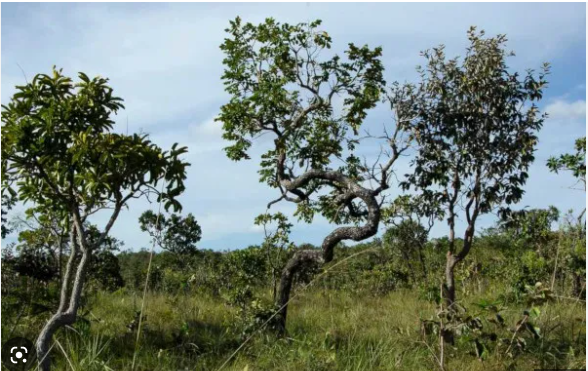
\includegraphics[width=.5\textwidth]{./imgs/img6.png}
\caption{Vegetação natural de cerrado.}

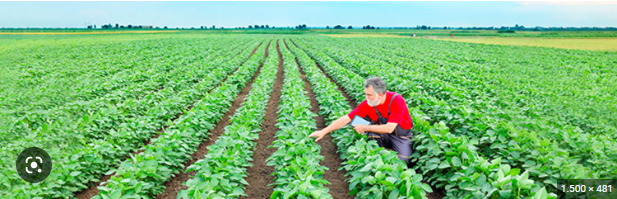
\includegraphics[width=.5\textwidth]{./imgs/img7.png}
\caption{Campo de cultivo de soja.}
\end{figure}

Considerando-se que sempre existe uma vegetação natural original onde se coloca um campo de cultivo, é correto
dizer que, na paisagem retratada na imagem em que aparece o campo de soja, há uma manipulação da energia pelo ser humano? Justifique.

\linhas{8}

\coment{Sim. Na paisagem retratada pela primeira imagem, uma formação natural está utilizando a
energia para crescer, enquanto, na segunda paisagem, ocorreu o plantio de soja, que
também vai utilizar a energia solar para crescer, mas de uma maneira
planejada pelo ser humano.}

\num{5} Desde os alimentos que são produzidos fora da zona urbana até a própria água -- que muitas vezes é extraída longe --, as cidades dependem muito do que é externo a elas., desde os alimentos que
são produzidos fora dos limites urbanos e até da própria água, que
muitas vezes é extraída longe da cidade. A seguir, marque com um X as ações capazes
de aproximar a cidade de suas necessidades.

\begin{boxlist}
\item Construção de hortas urbanas. \coment{X}

\item Drenagem total de rios e pântanos.

\item Criação de florestas urbanas. \coment{X}

\item Expansão da cidade.
\end{boxlist}

\coment{A construção de hortas urbanas aproxima a produção de alimentos dos
moradores das cidades, e as florestas urbanas promovem melhoria geral da qualidade
do ar e ainda garantem a preservação de nascentes. Essas duas ações aproximariam as cidades de suas necessidades.}

\num{6} A manutenção natural do calor na atmosfera terrestre é chamada de
\textbf{efeito estufa}. O esquema a seguir ajuda a entender como se dá esse processo.

\begin{figure}[htpb!]
\includegraphics[width=3.07283in,height=3.91428in]{https://br.freepik.com/vetores-gratis/o-efeito-estufa-com-luz-solar-para-casa-verde_16456035.htm#query=greenhouse%20effect&position=5&from_view=search&track=ais}
\end{figure}

Com base nesse esquema, explique como ocorre o efeito estufa no planeta Terra.

\linhas{8}

\coment{O efeito estufa é a retenção do calor realizada pela atmosfera terrestre e
seus componentes. A radiação solar atinge o planeta, atravessa a atmosfera, e parte, quando é refletida pela superfície, é retida pela própria atmosfera. Com isso, mantém-se o calor na superfície do planeta.}

\num{6} Leia os textos a seguir.

\textbf{TEXTO 1}
\begin{quote}
\textbf{O que é o aquecimento global?}

Trata-se do aumento da temperatura média dos oceanos e da camada de ar próxima à superfície terrestre. O aquecimento global se desenvolve conforme aumentam as emissões de determinados gases para a atmosfera -- o principal é o gás carbônico.

\fonte{Fonte de pesquisa: WWF. O que é o aquecimento global? Disponível em:
\emph{wwf.org.br/natureza\_brasileira/reducao\_de\_impactos2/clima/mudancas\_climaticas2/}.
Acesso em: 26 fev. 2023.}
\end{quote}

\textbf{TEXTO 2}
\begin{quote}
\textbf{Efeito estufa}

A queima de combustíveis fósseis (gás natural, carvão mineral e petróleo) e o desmatamento de regiões tropicais são as principais causas antropogênicas (causadas pelo ser humano) que contribuem com as emisões de gases do efeito estufa.

Os combustíveis fósseis são queimados, principalmente, pelas termelétricas, pelas indústrias e por alguns meios de transporte (automóveis, ônibus e aviões, por exemplo).

Já o desmatamento contribui com o efeito estufa porque libera as grandes reservas de carbono que as florestas representam, armazenado em biomassa florestal.

\fonte{Fonte de pesquisa: IPAM Amazônia. Quais são as principais fontes de gases de efeito estufa decorrentes das atividades humanas? Disponível em:
\emph{https://ipam.org.br/entenda/quais-sao-as-principais-fontes-de-gases-de-efeito-estufa-decorrentes-das-atividades-humanas-2/}. Acesso em: 26 fev. 2023.}
\end{quote}

Com base no texto e em seus conhecimentos, você afirmaria que o aquecimento global é a intensificação do
efeito estufa? Comente.

\linhas{6}

\coment{O efeito estufa é um fenômeno natural importantíssimo para a manutenção da vida na Terra e é ocasionado pela presença de determinados gases na atmosfera. O problema do aquecimento global é que, com a emissão descontrolada de gases do efeito estufa, esse fenômeno intensifica-se e aquece o planeta além do necessário.}

\num{8} Os últimos trezentos anos marcaram uma profunda mudança na relação da
sociedade com a natureza, pois, a partir das revoluções
industriais, o homem passou a consumir os recursos naturais em uma
velocidade maior do que aquela com que a natureza consegue se renovar. 
Novas necessidades surgiram, e as necessidades do ser humano
passaram a ser todas intermediadas pela indústria e pautadas no
consumismo de produtos que logo são descartados. A necessidade de
produzir mais e mais implica emprego de grandes volumes de
energia, obtidos principalmente a partir da queima de
combustíveis fósseis, cuja queima emite gás carbônico, o qual intensifica a retenção de calor na atmosfera,
o que altera os ciclos naturais do clima.
Quanto a esse contexto, que alternativas o ser humano tem para não destruir seu próprio hábitat?

\linhas{10}

\coment{Resposta pessoal. Espera-se que os alunos reflitam sobre a situação ruim em que a humanidade se encontra e tentem pensar em maneiras de alterar o quadro enquanto é tempo.}


\num{9} Indique soluções plausíveis para as causas das ilhas de calor.

\begin{escolha}
\item Excesso de construções.

\linhas{5}

\coment{Melhoria da ventilação natural de prédios e bairros; construção de áreas de lazer abertas; investimento em arquitetura verde.}

\item Ausência de vegetação contínua.

\linhas{5}

\coment{Reflorestamento; arborização urbana; valorização do paisagismo.}
\end{escolha}


\num{10} A vida útil média de um telefone celular é, atualmente, de dois anos, mas especialistas apontam para o fato de que, se não fosse a obsolescência programada, um celular duraria de 12 a 15 anos. Comente sobre os impactos da obsolescência programada:

\begin{escolha}
\item  na utilização de energia pelas indústrias.

\linhas{4}

\coment{Como os produtos duram pouco, é preciso que se produza com maior
frequência, o que gera mais gasto energético.}

\item  na exploração de recursos naturais.

\linhas{4}

\coment{A produção precisa suprir a pouca durabilidade dos produtos, e isso faz com que seja extraído da natureza
um volume maior de recursos.}

\item na vida das pessoas.

\linhas{4}

\coment{Há impacto negativo na vida das pessoas, que não conseguem realizar suas
tarefas quando os produtos estragam, além de que precisam desembolsar mais
dinheiro para garantir o acesso a itens básicos.}
\end{escolha}

\colorsec{Treino}

\num{1} Leia o texto.

\begin{quote}
\textbf{Instalação de painéis solares cresce 560\% no País}

Que tal você mesmo gerar a energia que consome em casa, a
partir da captação da luz solar? Melhor ainda: que tal vender para a
distribuidora {[}...{]} a energia excedente? {[}...{]}

Segundo a Agência Nacional de Energia Elétrica (Aneel), nos
últimos dois anos, a instalação de painéis solares para geração própria
de energia elétrica aumentou mais de 560\%. O número saltou de 7.400
para 49 mil unidades em todo o Brasil. São instalações em residências,
empresas e indústrias.

{[}...{]}

\fonte{Jornal da USP. Instalação de painéis solares cresce 560\% no País.
Disponível
em: \emph{https://jornal.usp.br/atualidades/instalacao-de-paineis-solares-cresce-560-no-pais/}.
Acesso em: 28 fev. 2023.}
\end{quote}

O impacto ambiental do tipo de produção elétrica citado se dá em razão

\begin{escolha}
\item
  do aumento de produção de painéis.
\item
  da eliminação de redes elétricas cabeadas.
\item
  do melhor aproveitamento da energia disponível.
\item
  da diminuição do consumo total de energia elétrica.
\end{escolha}

\coment{BNCC: EF09GE18 -- Identificar e analisar as cadeias industriais e de
inovação e as consequências dos usos de recursos naturais e das
diferentes fontes de energia (tais como termoelétrica, hidrelétrica,
eólica e nuclear) em diferentes países.

a) Incorreta. Se for considerado apenas o aumento da produção de painéis,
haveria um impacto potencialmente negativo em razão da exploração dos
recursos naturais.
b) Incorreta. No texto, cita-se que existem 49.000 painéis
solares domésticos, o que é insuficiente para suprir toda a demanda
energética do país, que tem mais de 200 milhões de habitantes.
c) Correta. A instalação de painéis solares permite o aproveitamento do
potencial energético local, já que são instalados em cima de casas para
poder captar a energia do Sol.
d) Incorreta. Os painéis não geram diminuição do consumo de energia; apenas
se tornam uma fonte a mais de eletricidade disponível.}

\num{2} Compare as duas tabelas a seguir.

%Paulo, criar uma tabela com estes dados:
%Título: Matriz energética mundial (2020)
%Carvão mineral 26,8%
%Petróleo e derivados 29,5%
%Gás natural 23,7%
%Nuclear 5,0%
%Hidráulica 2,7%
%Biomassa 9,8%
%Outras 2,5%
%Fonte de pesquisa: Empresa de Pesquisa Energética. Disponível em: https://www.epe.gov.br/pt/abcdenergia/matriz-energetica-e-eletrica. Acesso em: 04 abr. 2023.

%Paulo, criar uma tabela com estes dados:
%Título: Matriz energética brasileira (2021)
%Carvão mineral 5,6%
%Petróleo e derivados 34,4%
%Gás natural 13,3%
%Nuclear 1,3%
%Hidráulica 11,0%
%Lenha e carvão vegetal 8,7%
%Derivados da cana-de-açúcar 16,4%
%Outras renováveis 8,7%
%Outras não renováveis 0,6%
%Fonte de pesquisa: Empresa de Pesquisa Energética. Disponível em: https://www.epe.gov.br/pt/abcdenergia/matriz-energetica-e-eletrica. Acesso em: 04 abr. 2023.

Observa-se que, no Brasil, a matriz energética

\begin{escolha}
\item
  segue tendências mundiais, apesar de alguns avanços.
\item
  não apresenta avanço em relação ao restante do mundo.
\item
  utiliza energia nuclear na mesma proporção que o restante do mundo.
\item
  não gera energia com base em fontes renováveis, como no restante do mundo.
\end{escolha}

\coment{BNCC: EF09GE18 -- Identificar e analisar as cadeias industriais e de
inovação e as consequências dos usos de recursos naturais e das diferentes fontes de energia (tais
como termoelétrica, hidrelétrica, eólica e nuclear) em diferentes países.

a) Correta. A matriz brasileira apresenta alguns avanços em relação à matriz mundial, mas a tendência nas duas é a mesma.
b) Incorreta. Há algumas melhorias, do ponto de vista da sustentabilidade, da matriz brasileira em relação à mundial.
c) Incorreta. A energia nuclear está menos presente no Brasil do que no mundo.
d) Incorreta. Há fontes renováveis tanto na matriz brasileira quanto na mundial.}

\num{3} Leia o texto.

\begin{quote}
\textbf{O que são mudanças climáticas?}

As mudanças climáticas antropogênicas, ou seja, aquelas causadas
pelo homem, estão associadas ao aumento da emissão de gases de efeito
estufa por queima de combustíveis fósseis (dos automóveis, das
indústrias, usinas termoelétricas), queimadas, desmatamento,
decomposição de lixo etc. A partir do final do século 18 (Revolução
Industrial) e na segunda metade do século 20, houve uma expansão da
produção industrial, o que gerou um grande aumento de emissões de gases
de efeito estufa na atmosfera. Existem fortes indícios de que o clima
está de fato mudando. As décadas de 1990 e 2000 foram as mais quentes
dos últimos 1.000 anos. As projeções do Painel Intergovernamental de
Mudanças Climáticas (IPCC) indicam que nos próximos 100 anos poderá
haver um aumento da temperatura média global entre 1,8°C e 4,0°C, e um
aumento do nível médio do mar entre 0,18 m e 0,59 m, o que pode afetar
significativamente as atividades humanas e os ecossistemas terrestres.

\fonte{INPE. Perguntas frequentes. O que são mudanças climáticas? Disponível em: \emph{www.inpe.br/faq/index.php?pai=9\#:~:text=A\%20partir\%20do\%20final\%20do,clima\%20est\%C3\%A1\%20de\%20fato\%20mudando}. Acesso em: 28 fev. 2023.}
\end{quote}

A relação entre gases do efeito estufa e mudanças climáticas é explicada pelo fato
de as emissões humanas passarem a compor

\begin{escolha}
\item
  uma interferência dissociada dos ciclos naturais.
\item
  a capacidade de resfriamento atmosférico.
\item
  o ciclo de crescimento florestal.
\item
  o sistema climático global.
\end{escolha}

\coment{BNCC: EF09GE18 -- Identificar e analisar as cadeias industriais e de
inovação e as consequências dos usos de recursos naturais e das diferentes fontes de energia (tais
como termoelétrica, hidrelétrica, eólica e nuclear) em diferentes países.

a) Incorreta. O fato de as emissões humanas estarem interferindo no clima
global mostra que há uma integração da sociedade com o ciclo climático
global.
b) Incorreta. Os gases do efeito estufa não têm capacidade de gerar
resfriamento atmosférico.
c) Incorreta. Apesar de poderem favorecer crescimento florestal, as
emissões de gases do efeito estufa têm seu maior impacto no aquecimento
atmosférico, estando também relacionadas à própria destruição florestal
existente, já que o desmatamento promove a emissão de gás carbônico.
d) Correta. As emissões de gases do efeito estufa se integraram à dinâmica
climática, pois o maior aquecimento atmosférico está alterando os ciclos
dos sistemas atmosféricos e terrestres como um todo.}


\chapter{SIMULADO 1}

\num{1} Leia o texto.

\begin{quote}
Carvão é o nome dado a diversas rochas sedimentares passíveis
de uso como combustível, constituídas de um material heterogêneo
originado de restos vegetais depositados em águas rasas, protegidos da
ação do oxigênio do ar. {[}...{]}

A extração do carvão pode ser em minas a céu aberto ou
subterrâneas, dependendo da profundidade em que se encontra a camada. As
minas a céu aberto exercem significativo impacto ambiental em razão dos
elementos químicos contidos no carvão, como o enxofre.

Numerosas áreas de mineração antigas no sul do Brasil, trabalhadas
em uma época em que a preocupação com o ambiente natural era muito menor
que atualmente, foram muito degradadas e precisaram ser recuperadas,
trabalho que vem sendo feito nas últimas décadas.

{[}...{]}

\fonte{Serviço Geológico do Brasil. Carvão mineral. Disponível em:
\emph{http://www.cprm.gov.br/publique/SGB-Divulga/Canal-Escola/Carvao-Mineral-2558.html}.
Acesso em: 28 fev. 2023.}
\end{quote}

É possível identificar que o principal impacto da extração de carvão se dá pela

\begin{escolha}
\item
  emissão local de fumaça.
\item
  geração de ilhas de calor.
\item
  exaustão do lençol freático.
\item
  remoção da estrutura superficial do solo.
\end{escolha}

\coment{BNCC: EF09GE18 -- Identificar e analisar as cadeias industriais e de
inovação e as consequências dos usos de recursos naturais e das diferentes fontes de energia (tais como termoelétrica, hidrelétrica, eólica e nuclear) em diferentes países.

a) Incorreta. A extração do carvão não produz massiva emissão de fumaça.
b) Incorreta. As ilhas de calor são fenômenos associados a grandes
  cidades.
c) Incorreta. Ao contrário da mineração de metais, não se utiliza água
  para a extração de carvão mineral.
d) Correta. Para extrair o carvão, toda a superfície acima da mina precisa
  ser removida.}

\num{2} Analise o esquema.

%\begin{figure}[htpb!]
%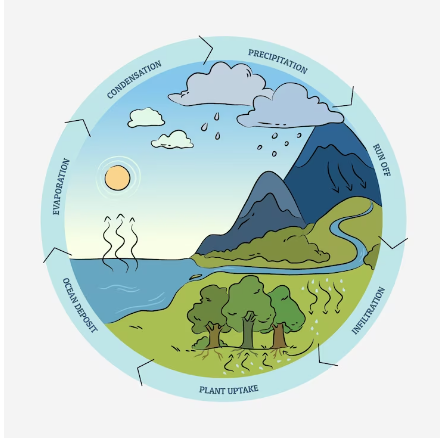
\includegraphics[width=4.58333in,height=4.56250in]{./imgs/img9.png}
%\caption{Fonte:
%https://br.freepik.com/vetores-gratis/informacoes-desenhadas-a-mao-sobre-o-ciclo-da-agua\_18980469.htm\#query=ciclo\%20da\%20agua\&position=1\&from\_view=keyword\&track=ais.}
%\end{figure}
%Paulo, trocar foto: https://br.freepik.com/vetores-gratis/desenho-a-mao-de-um-ciclo-de-agua-de-design-plano_18773933.htm#query=informacoes%20desenhadas%20a%20mao%20sobre%20o%20ciclo%20da%20agua&position=2&from_view=search&track=ais

No ciclo da água, a absorção de energia ocorre

\begin{escolha}
\item
  no escoamento.
\item
  na precipitação.
\item
  na condensação.
\item
  na evaporação.
\end{escolha}

\coment{BNCC: EF09GE18 -- Identificar e analisar as cadeias industriais e de
inovação e as consequências dos usos de recursos naturais e das diferentes fontes de energia (tais como termoelétrica, hidrelétrica, eólica e nuclear) em diferentes países.

a) Incorreta. O escoamento é orientado pela força da gravidade, e não pela
  energia solar.
b) Incorreta. A precipitação é o efeito da perda de calor por parte das
  nuvens, pois, ao perder calor, o vapor de água condensa-se em pequenas
  gotículas formando nuvens e posteriormente chuva.
c) Incorreta. Ao perder calor, o vapor de água condensa-se em pequenas
  gotículas formando nuvens e posteriormente chuva;
d) Correta. A evaporação é o efeito do ganho de calor (por meio da absorção da energia solar) por parte da água
  líquida, o que gera sua evaporação..}

\num{3} Leia o texto.

\begin{quote}
\textbf{Capacidade de geração de energia eólica deve bater recorde neste ano}

O Brasil registra, até fevereiro [de 2023], 890 parques eólicos instalados em 12 estados brasileiros. Eles somam 25,04 gigawatts (GW) de capacidade instalada em operação comercial, que beneficiam 108,7 milhões de habitantes.

Desse total, 85\% estão na Região Nordeste. De acordo com a Associação Brasileira de Energia Eólica (Abeeólica), até 2028 o Brasil terá 44,78 GW de capacidade instalada desse tipo de energia, cuja participação na matriz nacional atinge, atualmente, 13,2\%. A eólica já responde hoje por 20\% da geração de energia [de] que o país precisa.

No ano passado, o setor bateu recorde de 4 GW instalados e, para este ano, a presidente executiva da Abeeólica, Elbia Gannoum, espera atingir novo recorde, superando esse número. “Encerrando 2023, estaremos com 29 GW de capacidade instalada. Essa é a nossa previsão em termos de potência, e isso é superior a R\$ 28 bilhões, porque cada gigawatt de eólica instalada é da ordem de R\$ 7 bilhões”, disse Elbia {[}...{]}.

\fonte{Alana Gandra. Agência Brasil. Capacidade de geração de energia eólica deve bater recorde neste ano. Disponível em:
\emph{https://agenciabrasil.ebc.com.br/economia/noticia/2023-04/capacidade-de-geracao-de-energia-eolica-deve-bater-recorde-neste-ano}.
Acesso em: 05 abr. 2023.}
\end{quote}

O texto demonstra que o Brasil

\begin{escolha}
\item
  está avançando na produção de energia de uma fonte renovável.
\item
  é dependente de um tipo de energia que não tem muito potencial no país.
\item
  produz mais energia eólica do que a de qualquer outro tipo.
\item
  tem aumentado a produção de energia de fonte não renovável.
\end{escolha}

\coment{BNCC: EF09GE18 -- Identificar e analisar as cadeias industriais e de
inovação e as consequências dos usos de recursos naturais e das
diferentes fontes de energia (tais como termoelétrica, hidrelétrica,
eólica e nuclear) em diferentes países.

a) Correta. O texto demonstra o aumento da produção de energia eólica, que é de uma fonte renovável.
b) Incorreta. O texto demonstra que o Brasil tem muito potencial para energia eólica.
c) Incorreta. O texto demonstra que a energia eólica ainda corresponde a uma parcela pequena da matriz energética brasileira.
d) Incorreta. O texto demonstra o aumento de produção de energia de uma fonte renovável.}

\num{4} Leia o texto.

\begin{quote}
\textbf{Cota racial}

Em vigor desde 10 de junho de 2014, a Lei 12.990 prevê uma cota de vagas para negros e pardos em concursos públicos, com o objetivo de reduzir as desigualdades sociais, econômicas e educacionais entre as raças e promover uma maior inclusão e diversidade nos cargos públicos.

\fonte{Jusbrasil. Entenda como funciona a "cota racial" para concursos públicos no Brasil. Disponível em: \emph{https://www.jusbrasil.com.br/artigos/entenda-como-funciona-a-cota-racial-para-concursos-publicos-no-brasil/243608268}. Acesso em: 04 maio 2023.}
\end{quote}

Tal como em vestibulares, as cotas nos concursos públicos buscam

a)  discriminar racialmente a população branca.

b)  conferir privilégios para minorias demográficas.

c)  compor uma política ampla de reparação histórica.

d)  estabelecer mecanismos de compensação para incapazes.

\coment{BNCC: EF09HI03 -- Identificar os mecanismos de inserção dos
negros na sociedade brasileira pós-abolição e avaliar os seus
resultados.

a)  Incorreta. As políticas de cotas não versam sobre a população
    branca; apenas beneficiam a população negra e mais pobre.
b)  Incorreta. Ainda que fosse uma política de privilégios, a população
    foco não é minoritária, pois os negros compõem maioria demográfica.
c)  Correta. As leis de cotas buscam reparar injustiças históricas
    cometidas contra a população negra, que, por exemplo, sequer teve
    direito a trabalho livre após o fim da escravidão, o que causou
    inúmeras consequências relacionadas à exclusão econômica dessa
    população. 
d)  Incorreta. Essa alternativa possui uma abordagem racista ao afirmar
    que a população negra é menos capaz que a população branca.}


\num{5} Leia o texto.

\begin{quote}
\textbf{ONGs apontam racismo em falta de políticas públicas em áreas de risco}

A falta de políticas públicas voltadas a atender à demanda da população negra e periférica que vive em áreas de risco ambiental –-- como nos locais atingidos por deslizamentos de terra no litoral Norte de São Paulo --- é uma opção das administrações públicas e demonstra racismo ambiental. A avaliação é de especialistas de duas organizações da sociedade civil, o Greenpeace e o Instituto Polis.

``[O racismo ambiental] está muito ligado à segregação e [à] exclusão em relação ao direito de ter o meio ambiente de determinada região equilibrado. A gente observa a escolha política, o critério para definir locais que vão ter políticas públicas. E elas não conseguem chegar sempre à população dos morros, negra e periférica'', afirma Rodrigo Jesus, da Campanha Clima e Justiça, do Greenpeace.

De acordo com ele, a falta de prioridade das populações negra e periférica demonstra ainda negligência. {[}...{]}

\fonte{Bruno Bocchini. Agência Brasil. ONGs apontam racismo em falta de políticas públicas em áreas de risco. Disponível em: \emph{https://agenciabrasil.ebc.com.br/geral/noticia/2023-02/ongs-apontam-racismo-em-falta-de-politicas-publicas-em-areas-de-risco}. Acesso em: 04 maio 2023.}
\end{quote}

A criação de canais de representação e participação popular da população
negra contribuiria para a diminuição de desastres ambientais de maneira
geral ao

a)  organizar os governos locais.
b)  valorizar pautas esquecidas no debate público.
c)  explicar os mecanismos dos desastres ambientais.
d)  adequar o orçamento dirigido a obras públicas pontuais.

\coment{BNCC: EF09HI04 -- Discutir a importância da participação da
população negra na formação econômica, política e social do Brasil.

a) Incorreta. Atualmente existe extensa estrutura jurídica que embasa
a organização dos governos, não sendo este o fator causador da baixa
expressão política da população periférica.
b) Correta. Por serem as mais afetadas e, ao mesmo tempo, as menos
representadas, as pautas da população negra são pouco discutidas no
debate público; assim, a criação de canais de expressão e participação
popular daria mais evidência às pautas que afetam a população negra e
periférica.
c) Incorreta. Os mecanismos de desastres ambientais já são bem conhecidos,
e o problema repousa nas atitudes que deveriam ser, mas não são tomadas para
evitá-los, o que se explica em parte por racismo institucional.
d) Incorreta. A questão pede uma contribuição para a solução do conjunto
dos problemas ambientais que afetam a população negra, e não intervenções
pontuais.


\chapter{SIMULADO 2}

\num{1} Leia o texto.

\begin{quote}
\textbf{O arado}

Por volta do ano 5000 a.C., o ser humano
teria deixado de vagar atrás de terras
para cultivo e já começava a domesticar
animais. Foi nesse contexto que surgiu um
instrumento feito com galhos bifurcados e
uma pedra afiada na ponta, que servia
para arar a terra. Segundo especialistas,
a invenção do arado é um marco da Revolução Agrícola, que permitiu o ser humano fixar-se em aldeias, aumentar sua produtividade e dar início a atividades comerciais.

\fonte{Fonte de pesquisa: Superinteressante. Arado. Disponível em: \emph{https://super.abril.com.br/comportamento/arado/}. Acesso em: 04 abr. 2023.}
\end{quote}

No contexto apresentado, o arado cumpria a função de

\begin{escolha}
\item
  otimizar o trabalho humano.
\item
  domesticar os animais.
\item
  criar redes de água.
\item
  limpar terrenos.
\end{escolha}

\coment{BNCC: EF09GE05 -- Analisar fatos e situações para compreender a
integração mundial (econômica, política e cultural), comparando as
diferentes interpretações: globalização e mundialização.

a) Correta. O arado começou a ser utilizado para diminuir o tempo gasto com o preparo e a semeadura do solo; assim  constitui um instrumento que
otimiza o trabalho humano, isto é, a transformação de recursos naturais
em produtos com valor de uso. b) Incorreta. O arado não foi usado para domestificar animais, mas começou a ser empregado com o auxílio de animais domesticados.
c) Incorreta. O arado é um instrumento de preparação do solo para plantio.
d) Incorreta. O arado é empregado em terrenos já disponibilizados ao
plantio.}

\num{2} Leia os textos.

\textbf{TEXTO 1}
\begin{quote}
\textbf{Processo de desindustrialização no Brasil se acentua}

A indústria brasileira dá sinais de que algo de errado acontece no
setor. Do início do ano [de 2021] até agora [ou seja, março de 2021], três gigantes multinacionais
anunciaram que vão abandonar o Brasil. A norte-americana Ford deixa o
mercado de fabricação de veículos nacional depois de mais de 100 anos. A
alemã Mercedes-Benz fecha a única fábrica no Brasil de carros de luxo. A
japonesa Sony fecha a fábrica em Manaus (AM) e abandona o mercado de
televisores, câmeras e aparelhos de áudio. Esse movimento mostra que o
País passa por um processo de desindustrialização, e não é de hoje, como
sugerem alguns números e apontam especialistas.

{[}...{]}

\fonte{Ferraz Jr. Jornal da USP. Processo de desindustrialização no Brasil se
acentua. Disponível em:
\emph{https://jornal.usp.br/atualidades/processo-de-desindustrializacao-no-brasil-se-acentua/}.
Acesso em: 22 fev. 2023.}
\end{quote}

\textbf{TEXTO 2}
\begin{quote}
\textbf{Exportações do agronegócio batem recorde em dezembro e no ano de 2021}

As exportações do agronegócio alcançaram valores recordes para o
mês de dezembro passado e também para o ano de 2021. Foram US\$ 9,88
bilhões, valor recorde para os meses de dezembro: 36,5\% superior aos
US\$ 7,24 bilhões de 2020. Em 2021, o total exportado com o agronegócio
resultou em US\$ 120,59 bilhões, alta de 19,7\%, em relação ao ano
anterior, conforme dados divulgados nesta quinta-feira [13/01/2022] pela
Secretaria de Comércio e Relações Internacionais (SCRI) do Ministério da
Agricultura, Pecuária e Abastecimento (Mapa).

{[}...{]}

\fonte{Ministério da Agricultura e Pecuária. Exportações do agronegócio batem recorde em dezembro e no ano de 2021. Disponível em: \emph{www.gov.br/agricultura/pt-br/assuntos/noticias/exportacoes-do-agronegocio-batem-recorde-em-dezembro-e-no-ano-de-2021}. Acesso em: 22 fev. 2023.}
\end{quote}

Associando-se os textos, é possível diagnosticar que, no contexto
globalizado atual, o Brasil tem se constituído como

\begin{escolha}
\item
  exportador de serviços e consumidor de \textit{commodities}.
\item
  investidor tecnológico e consumidor de industrializados.
\item
  exportador de produtos básicos e consumidor de tecnologia.
\item
  centralizador da indústria global e exportador de produtos básicos.
\end{escolha}

\coment{BNCC: EF09GE05 -- Analisar fatos e situações para compreender a
integração mundial (econômica, política e cultural), comparando as
diferentes interpretações: globalização e mundialização.

a) Incorreta. O setor de serviços constitui destaque interno no Brasil.
b) Incorreta. A desindustrialização demonstra que o Brasil passa por um
  processo de perda de tecnologia, seja por perder empresas detentoras
  de tecnologias, seja por não investir na tecnologia, setor que anda
  lado a lado com o desenvolvimento industrial.
c) Correta. O recorde de exportações agrícolas revela o pleno
  desenvolvimento do setor no país, o que mostrar que o Brasil tem se
  especializado na produção de itens básicos classificados como
  matéria-prima (\textit{commodities}), e essa configuração econômica
  contribui para o país ficar dependente de tecnologia externa, já que o
  desenvolvimento tecnológico, mesmo para máquinas agrícolas, parte do
  setor industrial.
d) Incorreta. Em um dos textos, menciona-se a perda crônica de empresas
  industriais.}

\num{3} 

\begin{quote}
\textbf{Sem fé, lei ou rei}
No século XVI, Pero de Magalhães (um cronista português) acreditava ter encontrado a chamada \textit{mácula original do silvícola brasileiro}. O cronista escreveu que os indígenas estavam fadados a não se destacar, o que se devia ao fato de que, na língua deles, não havia F, L ou R, de modo que não tinham nem fé, nem lei, nem rei.

\fonte{Terras indígenas no Brasil. Sem fé, lei ou rei. Disponível em:
\emph{https://terrasindigenas.org.br/noticia/30695}. Acesso em: 22 fev. 2023.}
\end{quote}

A fala de Pero Magalhães é um demonstrativo de que a sociedade tida como
correta, em sua visão, teria como base

\begin{escolha}
\item
  a ausência da figura do rei.
\item
  a adoção da língua portuguesa.
\item
  a ideia de proteção ambiental dos indígenas.
\item
  as características políticas e sociais da Europa.
\end{escolha}

\coment{BNCC: EF09GE06 -- Associar o critério de divisão do mundo em Ocidente e
Oriente com o Sistema Colonial implantado pelas potências europeias.

a) Incorreta. Não apenas a ausência da figura do monarca é criticada, mas
também a ausência da fé cristã e da lei europeia.
b) Incorreta. O centro da visão colonialista não estava na língua falada,
mas nas características culturais diferenciadas dos povos indígenas.
c) Incorreta. A fala do cronista do português não se caracteriza por um tom de cuidado com os indígenas.
d) Correta. A monarquia, a fé cristã como instituição de estado e
a legislação portuguesa são encaradas como base de uma civilização
correta na fala de Pero Magalhães, motivo pelo qual ele critica a ausência
desses elementos entre os indígenas.}

\num{4} Analise o mapa.

\begin{quote}
\textbf{Ilú Obá De Min}

A associação Ilú Obá De Min é uma entidade sem fins lucrativos de São Paulo que tem como foco o trabalho com culturas de matriz africana, afro-brasileira e a valorização da mulher. Fundada em 2004 pelas percussionistas Beth Beli, Adriana Aragão e Girlei Miranda, a associação se tornou uma pessoa jurídica em 2006. Seu principal objetivo é preservar e divulgar a cultura negra no Brasil e fortalecer a participação e representatividade das mulheres negras. O projeto mais reconhecido da entidade é o Bloco Afro Ilú Oba De Min, cuja bateria é formada exclusivamente por mulheres. Desde 2005, o bloco realiza cortejos pelas ruas de São Paulo, honrando e celebrando a cultura afro-brasileira, além de destacar a participação e protagonismo feminino. Os cortejos do Bloco são uma grande intervenção cultural que promove a cultura negra, a cultura popular e a participação ativa das mulheres na sociedade por meio da arte. A iniciativa também traz para as áreas urbanas diversas manifestações da cultura negra, como o maracatu, batuque, coco, jongo, entre outras.

\fonte{Fonte de pesquisa: Ilú Obá De Min. Quem somos. Disponível em: \emph{https://iluobademin.com.br/institucional/quem-somos/}. Acesso em: 06 mar. 2023.}
\end{quote}

As ações executadas pela associação Ilú Obá De Min objetivam

a)  naturalizar as expressões culturais negras como identidade
    sociocultural.
b)  dramatizar as expressões culturais negras como meras atitudes
    lúdicas.
c)  diferenciar as expressões culturais negras como práticas
    estrangeiras.
d)  promover atos de protesto pontuais contra o racismo persistente.

\coment{BNCC: EF09GE03 -- Identificar diferentes manifestações
culturais de minorias étnicas como forma de compreender a multiplicidade
cultural na escala mundial, defendendo o princípio do respeito às
diferenças.

a)  Correta. A construção de projetos culturais de matrizes
    afro-brasileiras demonstra que as manifestações culturais promovidas
    pela associação têm como objetivo resgatar e consolidar uma
    identidade cultural própria da população negra.
b)  Incorreta. Os projetos desenvolvidos não têm como foco o
    divertimento, e sim a construção de práticas que representam a
    socialização da população negra em uma matriz cultural de origem
    africana.
c)  Incorreta. A associação busca a naturalização e a cotidianização das
    expressões culturais negras, o que promoveria maior integração
    dessas práticas com a cultura nacional.
d)  Incorreta. O objetivo da associação é a valorização das expressões
    culturais negras, que não são utilizadas como uma forma de
    contestação da ordem, mas como instrumento de consolidação de
    práticas socioculturais de origem africana}

\num{5}

\begin{quote}
\textbf{Brasil é líder em mortes de ambientalistas na última década}

Nos últimos 10 anos, o Brasil liderou o ranking mundial de assassinatos de defensores e defensoras do meio ambiente. De acordo com registros globais de 2012 a 2021, das 1.733 mortes, 342 ocorreram no país, representando quase 20\% do total. Entre as vítimas estão Maria José Rodrigues, de 78 anos, e seu filho José do Carmo Correa Junior, que foram esmagados por uma palmeira derrubada por um trator enquanto coletavam coco de babaçu em Penalva, Maranhão, em novembro de 2021. O tratorista estava desmatando uma área que já havia sido assegurada para uma comunidade tradicional, mas que estava sendo invadida a mando de um fazendeiro que, segundo denúncias dos moradores, pretendia plantar capim no terreno.

\fonte{Fonte de pesquisa: Nádia Pontes. G1. Brasil é líder em mortes de ambientalistas na última década. Disponível em: \emph{https://g1.globo.com/meio-ambiente/noticia/2022/09/29/brasil-e-lider-em-mortes-de-ambientalistas-na-ultima-decada.ghtml}. Acesso em: 04 maio 2023.}
\end{quote}

Qual das alternativas sintetiza as causas de violência contra
ambientalistas como as relatadas?

a)  Invasão de terras públicas.

b)  Disputa por recursos naturais.

c)  Roubo de produção agropecuária.

d)  Desregulamentação do extrativismo.

\coment{BNCC: EF09HI26 -- Discutir e analisar as causas da violência
contra populações marginalizadas (negros, indígenas, mulheres,
homossexuais, camponeses, pobres etc.) com vistas à tomada de
consciência e à construção de uma cultura de paz, empatia e respeito às
pessoas.

a)  Incorreta. Não há menção no texto à invasão de terras públicas como
    causa de violência.
b)  Correta. As mortes ocorridas em área previamente destinada ao
    extrativismo tradicional demonstram que disputas pelos recursos
    naturais são causas evidentes da violência rural.
c)  Incorreta. Não há menção no texto à prática de roubo da produção
    agropecuária como causa de violência.
d)  Incorreta. No texto, fica claro que a área onde ocorreram as mortes
    era destinada ao extrativismo, ou seja, existe regulamentação da
    atividade.}

\chapter{SIMULADO 3}

\num{1} Leia o texto.

\begin{quote}
\textbf{O caso de injustiça envolvendo a modelo Babiy Querino e a falha na identificação por foto}

Em 2017, a vida de Barbara Querino, então com 22 anos, foi drasticamente alterada por um reconhecimento 
fotográfico irregular. A modelo e dançarina, conhecida como Babiy, foi fotografada por policiais militares 
no dia em que seu irmão e primo foram presos, apesar de não ter qualquer envolvimento com o crime. A foto 
circulou em grupos de WhatsApp e páginas do Facebook, que a apresentaram falsamente como membro de uma 
quadrilha de assaltantes de carros atuando na zona sul de São Paulo. Em janeiro de 2018, Babiy foi presa 
sob acusação de ter participado de dois roubos em setembro de 2017, e permaneceu na prisão por 1 ano e 8 
meses, apesar de apresentar provas da sua inocência. Em 2020, a dançarina finalmente foi absolvida de todas 
as acusações.

\fonte{Caê Vasconcelos. Ponte. Por que tantos negros são alvo de prisão injusta com base em reconhecimentos. Disponível em: \emph{https://ponte.org/por-que-tantos-negros-sao-alvo-de-prisao-injusta-com-base-em-reconhecimentos/}. Acesso em: 10 mar. 2023.}
\end{quote}

Acontecimentos como o relatado são um claro desrespeito à "Declaração
universal dos direitos humanos" porque contrariam o princípio de que ninguém será

a)  mantido em escravidão ou servidão.

b)  preso, detido ou exilado arbitrariamente.

c)  submetido à tortura nem a tratamento cruel.

d)  privado de sua nacionalidade arbitrariamente.

BNCC: EF09HI16 -- Relacionar a Carta dos Direitos Humanos ao processo de
afirmação dos direitos fundamentais e de defesa da dignidade humana,
valorizando as instituições voltadas para a defesa desses direitos e
para a identificação dos agentes responsáveis por sua violação.

a) Incorreta. O texto trata de uma prisão injustas, e não de fatos
análogos à escravidão.
b) Correta. A modelo mencionada no texto foi presa, sem ter praticado
nenhum crime, com base em supostas provas forjadas pelas forças policiais, o
que contraria um dos artigos da ``Declaração universal dos direitos
humanos'', de que ninguém será arbitrariamente preso ou detido ou
exilado.
c) Incorreta. Não há menção a tortura no texto.
d) Incorreta. Não se trata de privação da nacionalidade.


\num{2} Leia o texto.

\begin{quote}
\textbf{Sistemas agroflorestais}

Os Sistemas Agroflorestais (SAFs) permitem aos agricultores familiares conciliar a produção de alimentos com a gestão das riquezas naturais de cada bioma. Na Bahia, {[}...{]} indígenas da etnia Pataxó, do território Barra Velha, município de Porto Seguro, a 629 km de Salvador, receberam do grupo ambiental Natureza Bela apoio para a implantação do corredor ecológico Monte Pascoal-Pau-Brasil, com a recuperação de uma área de mais de 50 hectares de terra, por meio da produção agroecológica de alimentos no Sistema Agroflorestal (SAF). {[}...{]}

\fonte{CONAFER. Agricultores Pataxó aliam produção de alimentos com reflorestamento via SAFs. Disponível em: \emph{https://conafer.org.br/povos-conafer-agricultores-pataxo-aliam-producao-de-alimentos-com-reflorestamento-via-safs/}. Acesso em: 11 mar. 2023.}
\end{quote}

Devido à prática de agricultura ecológica, a população Pataxó necessita,
primordialmente, de

a)  empréstimos bancários.

b)  qualificação na área industrial.

c)  áreas completamente florestadas.

d)  território disponível para plantio.

a) Incorreta. Apesar de empréstimos comporem quase sempre o circuito da
agricultura, a prática agroecológica por si não precisa de empréstimos
para ser efetivada.
b) Incorreta. Como o contexto fala de expansão de cultivos, tal alternativa
não se impõe como uma necessidade.
c) Incorreta. Como se mencionam cultivos, as áreas totalmente florestadas
não seriam úteis.
d) Correta. A população Pataxó precisa de áreas para o plantio, já que,
conforme o texto, estão desenvolvendo cultivos agrícolas.